\documentclass[frenchb,10pt,usenames,dvipsnames]{beamer}
\usepackage{../mypresentationstyle}
\graphicspath{{../images/}}
\newcommand{\thetitle}{Assembl�e G�n�rale\\Projet ANR SoDUCo\\(Social Dynamics in Urban Context)}
\title{\thetitle}
\subtitle{Open tools, models, and data - Paris and its suburbs, 1789-1950}

\author{\vspace{4cm}}

\date{01 octobre 2020}
\hypersetup{
  pdftitle={Projet ANR SoDUCo (Social Dynamics in Urban Context) - Presentation ANR - 2020},
  pdfsubject={\thetitle},
  pdfkeywords={Sciences ouvertes, interdisciplinarit�, sciences de l'information g�ographique, sciences humaines et sociales, syst�mes complexes et mod�les de simulation},
  pdfproducer={Latex with hyperref},
  pdfcreator={pdflatex},
  pdfauthor= {Julien Perret},
  colorlinks
}

\titlegraphic{
  \vspace{3.2cm}
  \centering
  
\includegraphics[height=0.05\textwidth]{logo_ign}\hfill
  
\includegraphics[height=0.05\textwidth]{logo_ehess}\hfill
  
\includegraphics[height=0.05\textwidth]{logo_epita}\hfill
  
\includegraphics[height=0.05\textwidth]{logo_an}\hfill
  
\includegraphics[height=0.025\textwidth]{logo_lnc}\\
  
\includegraphics[height=0.24\textwidth]{logo_soduco}
}
 
\begin{document}

\maketitle

\begin{frame}
  \frametitle{Ordre du jour}
  \hypertarget{odj}{}
  \begin{description}[align=left,labelwidth=1cm]
  \item[1] Point avancement du projet
  \item[2] Point d�penses du projet
  \item[3] Point recrutements du projet
  \item[4] Point Communication autour du projet
  \item[5] R�daction des rapports de mi-projet
  \item[6] Accord de consortium
  \item[7] Point Collaboration potentielle BnF / EPFL ?
  \item[8] Points divers
  \end{description}
\end{frame}

\begin{frame}
  \frametitle{Projet ANR SoDUCo : avancement}
%  Open tools, models, and data - Paris and its suburbs, 1789-1950\\
  \begin{figure}[htbp]
    \begin{center}
      
\includegraphics[width = 0.68\textwidth]{schema}
      \caption{Les t\^aches du projet SoDUCo}
      \label{fig:soduco}
    \end{center}
  \end{figure}
\end{frame}

\begin{frame}
  \frametitle{Projet ANR SoDUCo : avancement}
\begin{table}[ht!]
\footnotesize
\centering
\resizebox{0.85\textwidth}{!}{\begin{tabular}{llllll}
\topline
\headcol
\bf Task&
\bf N\textdegree&
\bf Name&
\bf Date&
\bf Type&
\bf Participants\\

\midline

\cellcolor{tableheadcolor}&0.1&Consortium agreement&T0&Document&\bf All\\
\rowcol
\cellcolor{tableheadcolor}&0.2&\soduco Website&every milestone&Website&\ign\\
\cellcolor{tableheadcolor}&0.3&Progress reports&every year&Document&\bf All\\
\rowcol
\cellcolor{tableheadcolor}&0.4&Minutes&every 6 months&Document&\bf All\\
\multirow{-5}{*}{\bf 0}
\cellcolor{tableheadcolor}&0.5&Repositories (code, data \& articles)&T3&Repositories&\ign\\

\midline

\rowcol
\cellcolor{tableheadcolor}{\bf 1.1}&1.1&Cartographic sources&T13&\dataset&\ehess, \natar\\
\cellcolor{tableheadcolor}{\bf 1.2}&1.2&Social sources&T15 \& T30&\dataset&\ehess, \natar\\
\rowcol
\cellcolor{tableheadcolor}&1.3.1&Sources integration \& diffusion tool&T7, T18 \& T36&\software&\ign, \ehess\\
\multirow{-2}{*}{\bf 1.3}
\cellcolor{tableheadcolor}&1.3.2&Metadata for directories and maps&T7, T18 \& T36&\dataset&\ign, \ehess, \natar\\

\midline

\rowcol
\cellcolor{tableheadcolor}&2.1.1&Extraction of topographic data&T4, T22&\software&\epita, \ign, \ehess\\
\multirow{-2}{*}{\bf 2.1}
\cellcolor{tableheadcolor}&2.1.2&Extraction of topographic data&T4, T22&\dataset&\epita, \ign, \ehess\\
\rowcol
\cellcolor{tableheadcolor}&2.2.1&Extraction of social data&T8, T26&\software&\epita, \ehess\\
\multirow{-2}{*}{\bf 2.2}
\cellcolor{tableheadcolor}&2.2.2&Extraction of social data&T8, T26&\dataset&\epita, \ehess\\
\rowcol
\cellcolor{tableheadcolor}&2.3.1&Spatio-Temporal geocoding&T8, T26&\software&\ign, \ehess\\
\multirow{-2}{*}{\bf 2.3}
\cellcolor{tableheadcolor}&2.3.2&Spatio-Temporal addresses&T8, T26&\dataset&\ign, \ehess\\
\rowcol
\cellcolor{tableheadcolor}{\bf 2.4}&2.4&Collaborative data correction&T12, T30&\software&\ign, \epita, \ehess\\

\midline

\cellcolor{tableheadcolor}{\bf 3.1}&3.1&Definition of phenomena&T6, T24&Document&\ehess, \natar\\
\rowcol
\cellcolor{tableheadcolor}&3.2.1&Analysis of co-evolution dynamics&T12, T30&Document&\ehess, \ign\\
\multirow{-2}{*}{\bf 3.2}
\cellcolor{tableheadcolor}&3.2.2&Co-evolution dynamics&T12, T30&\software&\ehess, \ign\\
\rowcol
\cellcolor{tableheadcolor}&3.3.1&Geo-historical co-visualisation&T12, T30&Document&\ign, \ehess\\
\multirow{-2}{*}{\bf 3.3}
\cellcolor{tableheadcolor}&3.3.2&Geo-historical co-visualisation&T12, T30&\software&\ign, \ehess\\
\rowcol
\cellcolor{tableheadcolor}{\bf 3.4}&3.4&Collaborative analysis and mapping&T24, T48&\software&\ign, \ehess\\

\bottomlinec
\end{tabular}}
%\vspace{.5em}
    \caption{Main deliverables for the \soduco project.}
    \label{deliverables}
\end{table}

\end{frame}

\begin{frame}
  \frametitle{Projet ANR SoDUCo : avancement}

\begin{figure}[ht!]
  %\input{gantt}
  \vspace*{-1em}
  \centering
  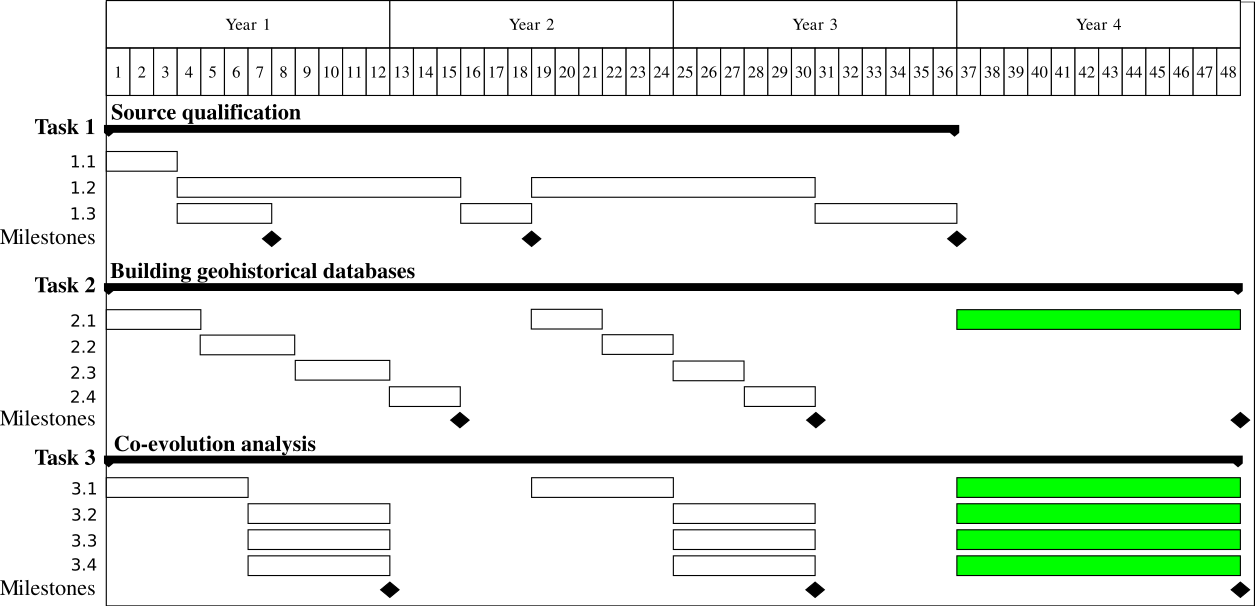
\includegraphics[width=\linewidth]{gantt.png}
  %\vspace*{.5em}
  \caption{Gantt diagram of the \soduco project.}
  \label{tasks}
  \vspace*{-1em}

\end{figure}
\end{frame}

\begin{frame}
  \frametitle{Projet ANR SoDUCo : d�penses}
  \begin{table}
  \vspace*{-1em}
\centering
{\footnotesize
\resizebox{0.85\textwidth}{!}{\begin{tabular}{llrrrrr}
\toprule
                                    &                  & \bign     & \behess   & \bepita   & \ban      & \bf{Total} \\
\cmidrule{2-7}
\multirow{5}{*}{\it Staff expenses} & PhD theses      & 36 m \textcolor{red}{(100 K\euro)}     & 36 m \textcolor{red}{(101 K\euro)}     &           &           & 201 K\euro \\
                                     & Interns         & 12 m ~~~~\textcolor{red}{(5 K\euro)}     & 12 m ~~\textcolor{red}{(28 K\euro)}     &  6 m  ~~\textcolor{red}{(45\% of 6 K\euro)}    &           &   36 K\euro \\ % IGN = 2 x 2646e / EHESS = 28000 / EPITA = .45 * 6 Ke = 36Ke
                                     & Engineers       & 24 m \textcolor{red}{(115 K\euro)}     &           & 17 m \textcolor{red}{(45\% of 80 K\euro)}     &           & 151 K\euro \\ % IGN = 114570e / EPITA = .45 * 80022e = 151Ke
                                     & Assitant. Pr.   &           &           & 12 m \textcolor{red}{(45\% of 70 K\euro)}     &           &  31 K\euro \\ % EPITA = .45 * 70438e = 31.7Ke
                                     & Professor             &           &           &  4 m \textcolor{red}{(45\% of 33 K\euro)}      &          &  15 K\euro \\ % EPITA = .45 * 33476e = 15.0Ke
\cmidrule{2-7}
                                     & Equipment       &  5 K\euro & 5 K\euro  &         &           &  10 K\euro \\
                                     & Digitisation    &           &           &           & 20 K\euro &  20 K\euro \\
                                     & Dissemination   & 10 K\euro & 5 K\euro &  45 \% of 1 K\euro  &           &  15 K\euro \\
                                     & Other services  & 20 K\euro  &           &           &           &  20 K\euro \\
\cmidrule{2-7}
\multicolumn{2}{l}{Total required (without overheads)} &255K\euro&139K\euro&85K\euro&20K\euro& 499 K\euro \\ % overheads = AN 1600 + IGN 20395 + EHESS 11162 + EPITA 0.45 * 28560e (12852e) = 46009e === 
\multicolumn{2}{l}{\bf Total required (with overheads)} &275K\euro&150K\euro&99K\euro&22K\euro& \bf 546 K\euro \\ % TOTAL = IGN 275337 + EHESS 150685 + EPITA 98773 + AN 21600
\toprule
  \end{tabular}
  }
} % small
\caption{\label{means} Scientific and technical means.}
\end{table}

\end{frame}

\begin{frame}
  \frametitle{Projet ANR SoDUCo : recrutement}
  \begin{description}[align=left,labelwidth=3cm]
  \item[Th�se IGN] \emph{Yizi Chen} recrut� en d�cembre 2019 - d�cembre 2022
  \item[Th�se EHESS] transform�e en PostDoc - � recruter
  \item[Ing�nieur IGN] � recruter avant septembre 2021
  \item[Stages/vacataires] ?
  \end{description}
\end{frame}

\begin{frame}
  \frametitle{Projet ANR SoDUCo : communication}
  \begin{description}[align=left,labelwidth=4cm]
  \item[FOSS4G 2019] Pr�sentation par Pierre-Andr� \& Bertrand
  \item[ACI 2019] Concours de carte + poster + r�sum�~\cite{Dumenieu2019engraved}
  \item[JoSIS 2019] Article de revue~\cite{Costes2019}
  \item[Pr�sentation EPITA] Pr�sentation par Pierre-Andr�
  \item[Sources aux SIG 2020] 2 soumissions aux colloque << des sources aux syst�mes d'information g�ographique : des outils pour la cartographie dans les humanit�s num�riques >>
  \item[ICDAR 2021] comp�tion accept�e pour l'analyse de cartes anciennes
  \item[Site web] Essayer de mettre en ligne ces informations et supports (si possible)
  \end{description}
\end{frame}

\begin{frame}
  \frametitle{Projet ANR SoDUCo : rapports}
  \begin{description}[align=left,labelwidth=3cm]
  \item[Objectifs] un document pour construire une vision commune, �tablir une strat�gie et la diffuser ?
  \item[Outils] overleaf, googledoc, autre ?
  \item[Planification] d�cembre 2020 ?
  \end{description}
\end{frame}

\begin{frame}
  \frametitle{Projet ANR SoDUCo : Accord de consortium}
  \begin{description}[align=left,labelwidth=3cm]
  \item[Premier jet envoy� � EPITA] mai 2020
  \item[Transmission du document � EHESS] septembre 2020
  \item[Planification] d�cembre 2020 ?
  \end{description}

\end{frame}

\begin{frame}[standout]

  Merci de votre attention !
  
\end{frame}

\appendix

\begin{frame}[allowframebreaks]{R�f�rences}
  \hypertarget{references}{}
  \setbeamerfont{bibliography item}{size=\tiny}
  \setbeamerfont{bibliography entry author}{size=\tiny}
  \setbeamerfont{bibliography entry title}{size=\tiny}
  \setbeamerfont{bibliography entry location}{size=\tiny}
  \setbeamerfont{bibliography entry note}{size=\tiny}
  \bibliographystyle{amsalpha}
  \bibliography{presentation}
\end{frame}

\end{document}
